\section{Einleitung}
In dem Versuch wird der Reinst-Germanium-Detektor näher betrachtet. Dazu werden wichtige Kenngrößen, wie das energetische Auflösungsvermögen und die spektrale Empfindlichkeit, des Detektors bestimmt. Im folgenden werden der Aufbau und die Funktionsweise des Ge-Detektors näher beschrieben.



\section{Theoretische Grundlage}
\label{sec:Theorie}
Der Germanium-Detektor ist ein wichtiges Messinstrument in der $\gamma$-Spektroskopie. Er gehört zu der Gruppe der Halbleiterdetektoren, welche ein sehr hohes Auflösungsvermögen im Vergleich zu Szintillationsdetektoren besitzten.



\subsection{Wechselwirkung von \texorpdfstring{$\gamma$}{}-Strahlung mit Materie}
Im folgenden werden der Wirkungsquerschnitt $\sigma$ und der Extinktionskoeffizient $\mu$ angegeben, sowie die drei dominierenden Wechselwirkungen von $\gamma$-Strahlung mit Materie erläutert.



\subsubsection{Der Wirkungsquerschnitt \texorpdfstring{$\sigma$}{} und der Extinktionskoeffizient \texorpdfstring{$\mu$}{}}
Der Wirkungsquerschnitt $\sigma$ ist ein Maß für die Wahrscheinlichkeit, dass eine Wechselwirkung zwischen der $\gamma$-Strahlung und dem Absorber stattfindet. $\sigma$ hat die Dimension einer Fläche und man kann sich diese als Zielscheibe vorstellen. \todo{man wegmachen} Es tritt also genau dann eine Wechselwirkung auf, wenn ein $\gamma$-Quant die Zielscheibe trifft. \\
Die Wahrscheinlichkeit $dW$ einer Wechselwirkung zwischen dem einfallenden Strahl ("Projektil") und dem Absorber ("Target") wird mit Hilfe der Abbildung \eqref{fig:WkeitWW} zu
\begin{align}
	dW = n\,\sigma\,dx
\end{align}
bestimmt. Daraus folgt das Absorbtionsgesetzt \todo{wirklich Absorbtionsgesetzt?}
\begin{align}
	N(D) = N_0 \exp(-n\,\sigma\,D) \ .
\end{align}
Darin ist $N_0$ die Anzahl der auftreffenden Quanten und $N(D)$ ist die Anzahl der austretenden Quanten. $n$ ist die Teilchendichte des Absorbers. Der Extinktionskoeffizient $\mu$ wird als
\begin{align}
	\mu = n\,\sigma
\end{align}
deffiniert. Sein reziproker Wert ist gleich der mittleren Reichweite $\overline{x}$ der $\gamma$-Quanten in Materie \cite[2]{V18}.

\begin{figure}
	\centering
	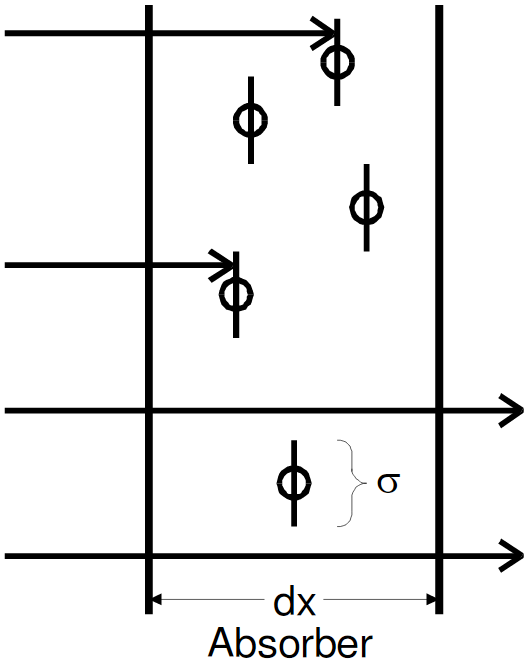
\includegraphics[width=0.3\textwidth]{Bilder/WkeitWW.png}
	\caption{Definition des Wirkungsquerschnitts: Die Pfeile kennzeichnen die Projektile welche auf das Target treffen \cite{V18}.}
	\label{fig:WkeitWW}
\end{figure}



\subsubsection{Der Photoeffekt}
Ein Photon kann ein Elektron aus der Atomhülle schlagen, dafür muss das Photon mindestens die Bindungsenergie $E_\text{B}$ des Elektrons besitzten. Bei diesem Vorgang wird die gesamte Energie $h\nu$ des Photons auf das Elektron übertragen. Das Elektron besitzt also eine kinetische Energie von
\begin{align}
	E_\text{kin} = h\nu - E_\text{B} \ .
\end{align}
Aus Energie-Impuls-Erhaltungsgründen kann dieser Prozess nur in der nähe eines Atomkerns stattfinden. Deshalb werden bevorzugt Elektronen aus der K-Schale ausgelöst (vgl. \cite[3]{V18}). Da sich das Atom nach dem Effekt in einem instabilen Zustand befindet, fallen Elektronen aus höheren Schalen in das enstandene "Loch". Dabei wird Röntgenstrahlung frei welche aber fast komplet in dem Absorber verbleibt. Deshalb kann gesagt werden, dass der Absorber die gesamte Energie des Photons absorbiert. \\
Der Wirkungsquerschnitt $\sigma_\text{Ph}$ des Photoeffekts kann zu
\begin{equation}
	\sigma_\text{Ph} \approx z^{\alpha}\,E^{\delta}
\end{equation}
bestimmt werden. Für den Energiebereich der bei natürlichen Strahlern vorkommt (E < 5\,MeV) ist $4 < \alpha < 5$ und $\delta = -3.5$\ .



\subsubsection{Der Compton- und der Thomson-Effekt}
Der Compton-Effekt ist die inelastische Streuung von Photonen an Elektronen. Das Photon gibt bei dem Stoß mit einem (schwachgebundenen) Elektron aus der Atomhülle einen Teil seiner Energie ab und wird aus der ursprünglichen Bahn herausgelenkt. Die Energie des gestreuten Photons kann Mithilfe des Energie-Impuls-Erhaltungssatzes zu
\begin{align}
	E_{\gamma'} = \frac{E_{\gamma}}{1 + \varepsilon\,(1-\cos(\psi_{\gamma})}
	\label{eqn:Egamma}
\end{align}
bestimmt werden. Dabei ist $E_{\gamma}$ die Energie des Photons vor dem Stoß und $E_{\gamma'}$ ist die Energie nach dem Stoß. $\varepsilon$ entspricht einer normierten Energie $\varepsilon = \frac{E_{\gamma}}{m_0\,c^2}$ und $\psi_{\gamma}$ ist der Streuwinkel des $\gamma$-Quants. Aus Formel \eqref{eqn:Egamma} folgt die Energie $E_\text{l}$ des gestoßenen Elektrons zu
\begin{align}
	E_\text{l} = E_{\gamma} - E_{\gamma'} = E_{\gamma} \frac{\varepsilon\,(1-\cos(\psi_{\gamma})}{1 + \varepsilon\,(1-\cos(\psi_{\gamma})} \ .
	\label{eqn:El}
\end{align}
Der Compton-Effekt ist eine unerwünschte Erscheinung, weil nur ein variierender Bruchteil der Energie des $\gamma$-Quants an den Detektor abgegeben wird (vgl. \cite[5]{V18}). Dadurch entsteht ein kontinuirliches Spektrum, welches schwer zu identifizieren ist. Der über alle Streuwinkel integrierte Wirkungsquerschnitt $\sigma_\text{Co}$ wurde von KLEIN und NISHINA hergeleitet und lautet:
\begin{align}
	\sigma_\text{Co} = \frac{3\,\sigma_\text{Th}}{4} \left( \frac{1+\varepsilon}{\varepsilon^2} \left[\frac{2+2\,\varepsilon}{1+2\,\varepsilon} - \frac{\ln(1+2\,\varepsilon)}{\varepsilon} \right] + \frac{\ln(1+2\,\varepsilon)}{2\,\varepsilon} - \frac{1+3\,\varepsilon}{(1+2\,\varepsilon)^2} \right)
\end{align}
Für sehr kleine Energien $(\varepsilon \ll 1)$ kann $\sigma_\text{Co}$ zu
\begin{align}
	\sigma_\text{Co} = \frac{3\,\sigma_\text{Th}}{4} \left(1 - 2\,\varepsilon + \frac{26}{5}\,\varepsilon^2 + \dots \right)
\end{align}
genähert werden. Für $\varepsilon \rightarrow 0$ geht der Compton-Wirkungsquerschnitt in den Thomsonschen Streuquerschnitt $\sigma_\text{Th}$ über.
\begin{align}
	\sigma_\text{Th} = \frac{8\,\pi}{3}\,r_\text{e}^2
\end{align}
$r_\text{e}$ wird als klassischer Elektronenradius bezeichnet.



\subsubsection{Die Paarbildung}
Bei der Paarbildung wird ein Photon annihilliert und ein Elektron-Positron-Paar erzeugt. Dieser Prozess kann nur in der nähe von einem Atomkern oder einem Elektron als Stoßpartner auftretten, weil sonst die Impulserhaltung nicht gilt. Mit dem Atomkern als Stoßpartner muss die Photonenergie größer als die doppelte Ruheenergie eines Elektrons sein, also
\begin{align*}
	E_{\gamma} > 2\,m_0\,c^2 \ .
\end{align*}
Damit die Paarbildung mit einem Elektron als Stoßpartner stattfinden kann muss das Photon die vierfache Ruheenergie eines Elektrons haben, also
\begin{align*}
	E_{\gamma} > 4\,m_0\,c^2 \ .
\end{align*}
Die kinetische Energie des entstandenen Elektron-Positron-Paares beträgt:
\begin{align}
	\overline{E_{\text{e}^-}} = \overline{E_{\text{e}^+}} = \frac{1}{2}(E_{\gamma} - m_0\,c^2)
\end{align}
Der Wirkungsquerschnitt der Paarbildung $\sigma_\text{Pa}$ hängt von der Kernladungszahl $z$ und der Abschirmung des Coulomb-Feldes ab. Im folgenden werden zwei Grenzfälle betrachtet. Wenn die Paarbildung in Kernnähe auftritt, also bei verschwindender Abschirmung wird der Wirkungsquerschnitt zu
\begin{align}
	&\sigma_\text{Pa} = \alpha\, r_\text{e}^2\, z^2\, \left(\frac{28}{9}\ln(2\,\varepsilon) - \frac{218}{27} \right) \\
	(\alpha = &\text{Sommerfeldsche Feinstrukturkonstante})
	\label{eqn:PaarVerschwindend}
\end{align}
bestimmt. Die Gleichung \eqref{eqn:PaarVerschwindend} ist in einem Energiebereich von $10 < E_\gamma < 25$ MeV gültig. \\
Wenn die Paarbildung am Rand der Elektronenhülle stattfindet, das Coulomb-Feld also vollständig abgeschirmt wird, ergibt sich folgende Gleichung
\begin{align}
	\sigma_\text{Pa} = \alpha\, r_\text{e}^2\, z^2\, \left(\frac{28}{9}\ln\frac{183}{\sqrt[3]{z}} - \frac{2}{27} \right) \ .
\end{align}
Diese ist aber erst ab 500 MeV gültig. \\
Bei der Paarbildung wird die gesamte Energie des Photons in dem Absorber deponiert. Allerdings kann nicht immer die gesamte Energie von dem Detektor gemessen werden, weil dazu Elektron und Positron in den Detektor fallen müssen. Passiert dies nicht, wird keine Energie gemessen. Auch verlieren Elektron und Positron durch Bremsstrahlung Energie, wodurch das Spektrum nach unten verbreitert wird.



\newpage
\subsection{Wirkungsweise eines Halbleiter-Detektors (Germanium-Detektor)}
Halbleiter-Detektoren werden häufig verwendet um ionisierende Strahlung nachzuweisen und die Energie der Strahlung zu bestimmen. Im folgenden wird der Germanium-Detektor für die $\gamma$-Spektroskopie genauer betrachtet. \\
Der wesentliche Bestandteil des Detektors ist eine Diode. Das bedeutet es gibt einen p- und einen n-dotierten Bereich. Diese Bereiche grenzen aneinander und können freie \todo{wirklich freie Ladungsträger?} Ladungsträger (Elektronen und Löcher) austauschen. Die Elektronen und Löcher rekombinieren in den unterschiedlich dotierten Bereichen. Zurück bleiben in der p-Schicht die ortsfesten Akzeptoren und in der n-Schicht die ortsfesten Donatoren \cite[10]{V18}. Diese bilden ein elektrisches Feld aus, wodurch die Elektronen und Löcher nicht mehr rekombinieren können und es entsteht eine ladungsträgerarme Zone. 



-es bildet sich ein E-Feld aus
-dadurch entsteht Ladungsträger arme Zone
-diese kann durch eine äußere Spannung vergrößert werden

\begin{figure}[H]
	\centering
	\begin{subfigure}[b]{0.49\linewidth}
		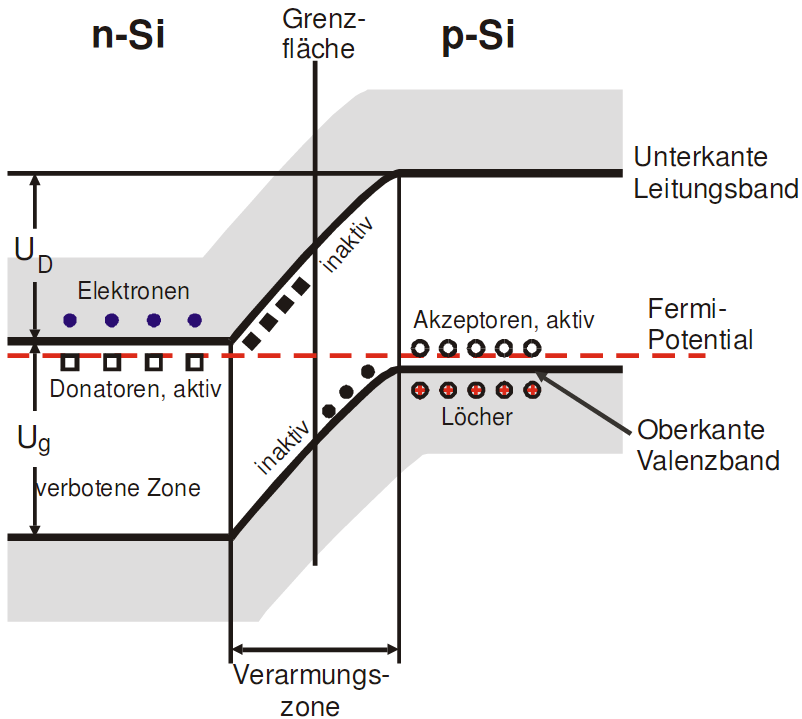
\includegraphics[width=\linewidth]{Bilder/V1.png}
		\caption{Potentialverhältnis ohne äußere Spannung.}
	\end{subfigure}
	\begin{subfigure}[b]{0.49\linewidth}
		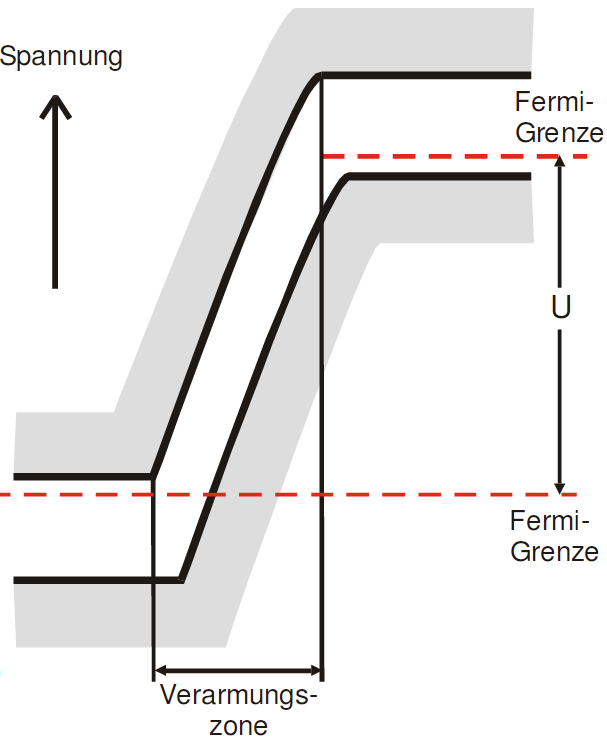
\includegraphics[width=\linewidth]{Bilder/V2.png}
		\caption{Potentialverhältnis mit äußere Spannung.}
	\end{subfigure}
	\caption{Schematische Darstellung der Potentialverhältnisse an einem pn-Übergang \cite{V18}.}
\end{figure}

-wenn ein y-Quant in die Verarmungszone eindringt, wird ein Energiereiches Elektron frei
-dieses stößt mit weiteren Elektronen im Valenzband und löst diese aus, dadurch entsteht eine Spannung welche gemessen wird
-






























\subsection{Fehlerrechnung}
Sämtliche Fehlerrechnungen werden mit Hilfe von Python 3.4.3 durchgeführt.
\subsubsection{Mittelwert}
Der Mittelwert einer Messreihe $x_\text{1}, ... ,x_\text{n}$ lässt sich durch die Formel
\begin{equation}
	\overline{x} = \frac{1}{N} \sum_{\text{k}=1}^\text{N} x_k
	\label{eqn:ave}
\end{equation}
berechnen. Die Standardabweichung des Mittelwertes beträgt
\begin{equation}
	\Delta \overline{x} = \sqrt{ \frac{1}{N(N-1)} \sum_{\text{k}=1}^\text{N} (x_\text{k} - \overline{x})^2}
	\label{eqn:std}
\end{equation}

\subsubsection{Gauß'sche Fehlerfortpflanzung}
Wenn $x_\text{1}, ..., x_\text{n}$ fehlerbehaftete Messgrößen im weiteren Verlauf benutzt werden, wird der neue Fehler $\Delta f$ mit Hilfe der Gaußschen Fehlerfortpflanzung angegeben.
\begin{equation}
	\Delta f = \sqrt{\sum_{\text{k}=1}^\text{N} \left( \frac{ \partial f}{\partial x_\text{k}} \right) ^2 \cdot (\Delta x_\text{k})^2}
	\label{eqn:var}
\end{equation}

\subsubsection{Lineare Regression}
Die Steigung und y-Achsenabschnitt einer Ausgleichsgeraden werden gegebenfalls mittels Linearen Regression berechnet.
\begin{equation}
	y = m \cdot x + b
	\label{eqn:reg}
\end{equation}
\begin{equation}
	m = \frac{ \overline{xy} - \overline{x} \overline{y} } {\overline{x^2} - \overline{x}^2}
	\label{eqn:reg_m}
\end{equation}
\begin{equation}
	b = \frac{ \overline{x^2}\overline{y} - \overline{x} \, \overline{xy}} { \overline{x^2} - \overline{x}^2}
	\label{eqn:reg_b}
\end{equation}
